% REMEMBER: You must not plagiarise anything in your report. Be extremely careful.

\documentclass{l4proj}

    
%
% put any additional packages here
%
\usepackage{hyperref}
\usepackage{booktabs}

\begin{document}

%==============================================================================
%% METADATA
\title{Automated Exercise and Solution Generation for an Algorithmics Course}
\author{Zoltan Sojtory}
\date{March 24, 2023}

\maketitle

%==============================================================================
%% ABSTRACT
\begin{abstract}
	With the rise of the COVID-19 pandemic, distance learning became the default overnight across all levels of education. This caused numerous challenges for educators, with one of the greatest being the introduction of online written examinations. Due to very limited monitoring capabilities, student collusion became rampant, undermining the academic integrity of these examinations. Automated exercise generation is a teaching method that aims to solve this by providing each student unique exam sheets with uniform difficulties. For the purpose of this project, I created a program which generates exercises and solutions for two common algorithms taught in introductory algorithmics courses: \textit{Dijkstra's algorithm} and the \textit{Knuth–Morris–Pratt algorithm}. While it may take considerable time for exam boards to approve the use of automatically generated exercises, I believe my program serves as a great resource for exam preparation or formative assessments. This is especially true considering that it can be easily expanded with other algorithms in the future.
\end{abstract}

%==============================================================================

% EDUCATION REUSE CONSENT FORM
% If you consent to your project being shown to future students for educational purposes
% then insert your name and the date below to  sign the education use form that appears in the front of the document. 
% You must explicitly give consent if you wish to do so.
% If you sign, your project may be included in the Hall of Fame if it scores particularly highly.
%
% Please note that you are under no obligation to sign 
% this declaration, but doing so would help future students.
%
%\def\consentname {My Name} % your full name
%\def\consentdate {20 March 2018} % the date you agree
%
\educationalconsent


%==============================================================================
\tableofcontents

%==============================================================================
%% Notes on formatting
%==============================================================================
% The first page, abstract and table of contents are numbered using Roman numerals and are not
% included in the page count. 
%
% From now on pages are numbered
% using Arabic numerals. Therefore, immediately after the first call to \chapter we need the call
% \pagenumbering{arabic} and this should be called once only in the document. 
%
% Do not alter the bibliography style.
%
% The first Chapter should then be on page 1. You are allowed 40 pages for a 40 credit project and 30 pages for a 
% 20 credit report. This includes everything numbered in Arabic numerals (excluding front matter) up
% to but excluding the appendices and bibliography.
%
% You must not alter text size (it is currently 10pt) or alter margins or spacing.
%
%
%==================================================================================================================================
%
% IMPORTANT
% The chapter headings here are **suggestions**. You don't have to follow this model if
% it doesn't fit your project. Every project should have an introduction and conclusion,
% however. 
%
%==================================================================================================================================
\chapter{Introduction}
\label{chap:intro}

% reset page numbering. Don't remove this!
\pagenumbering{arabic} 

\section{Motivation}

Leading up the COVID-19 pandemic, online teaching platforms had already become quite popular in higher education institutions due to convenient features such as lecture recordings, quizes and online communication channels. As distance teaching had to be adopted overnight in accordance with government guidance, these services became essential for delivering course material and assessments. However, not only did these platforms become incredibly overloaded, fatal issues also began to emerge. Arguably the greatest challenge educaters started facing was how to conduct summative assessments (specifically written examinations). This is because traditional methods in an at-home examination setting would lead to increased student collusion, jeopardising academic integrity, while online monitoring during examinations is very difficult and also possibly ethically unsound. Automated exercise generation aims to address this issue by providing each student an examination paper with unique exercises of uniform difficulty, eliminating possible collusions without using only monitoring procedures. Although in person examinations are underway once again (in the United Kingdom at least), many faculties still prioritise online assessments due to scheduling constraints, venue scarcities and/or student preferences, thus the demand for automated exercise generation.

Previous work in automated exercise generation has been done in contexts including satisfiability problems \cite{Hoz21}, embedded systems  \cite{Sad12}, and data science \cite{Kot19} (further explored in \autoref{chap:back}), however not much research exists on graph and string algorithms typically taught in algorithmics courses. Generating for these algorithms requires in-depth design (\autoref{chap:des}), as this process is non-trivial, meaning that completely random generation will result in exercises of varying difficulties, violating academic integrity in a different way. This is what separates automated exercise generation from existing solutions on online platforms, which mostly deal with trivial generations.

For the purpose of this project, two algorithms were selected (one graph and one string to have an example of each) for which exercises and solutions would be generated. This was done to set a baseline for what is required in order to generate exercises of uniform difficulty, such that it can be replicated for other algorithms in this field of study. The following algorithms were chosen:
\begin{itemize}
	\item
	\textbf{Dijkstra's algorithm} for finding the shortest path between two vertices in a weighted graph. The exercise generated asks students to identify the shortest paths from a given a vertex to all other vertices in a weighted graph. (ref)
	\item
	The \textbf{Knuth–Morris–Pratt (KMP) algorithm} for string seach. For this exercise, students are required to build the border table of a given string, so that the KMP algorithm can be applied to search for a string. (ref)
\end{itemize}
The reason these specific algorithms were chosen is because they are popular amongst computing scientists (usually taught in undergraduate algorithmics courses), so that they have a familiar point of reference when they are analysing the generation algorithms. Even though the selected algorithms are not overly complex, this does not directly translate to the complexity of the generation algorithms (it is considerably more difficult to generate than to solve). 

Since the project deals with exercises being generated from scratch, it follows naturally to provide automatically generated solutions for said exercises as well. This process is taken one step further, by providing step-by-step solutions, allowing students to trace the way in which their unique exercise is to be solved. Solution generation is highly desired, as teachers would have to provide solutions for each individual exercise manually otherwise. This would defeat one of the main purposes of \emph{automatically} generating exercises as opposed to \emph{manual} generation, being the time taken to design and mark examination papers for a given cohort of students.

\section{Aims}
\label{sec:aim}

Considering the aforementioned motivations, the aim of this project is to design generation algorithms for the selected exercises and then build a program which lets educators generate large numbers of exercises (along with their solutions) through these algorithms. It is important to mention that there exist two main characteristics of these algorithms:
\begin{enumerate}
	\item
	The extent to which the generated exercises reduce collusion between students.
	\item
	The extent to which the generated exercises require the same workload to solve.
\end{enumerate}
There is a tradeoff between \emph{1.} and \emph{2.}, where one end of the spectrum is identical examination papers resulting in perfectly identical workloads but high collusion, whereas the other end is completely randomly generated exercises which eliminate collusion, but have drastically different difficulties. Therefore, the main goal of the project is to find a balance between \emph{1.} and \emph{2.} in a way that maximises academic integrity.

Once the program is operational, two separate evaluations will be conducted. One will focus on the usability of the program by surveying computing science lecturers, and the other will gain insight from third year computing science students on the generated exercises and solutions themselves. The combined results from these two user studies should highlight the extent to which the trade-off problem was successfully solved, as well as gather a general consensus about automated exercise and solution generation.

\section {Dissertation Outline}

This dissertation is comprised of the following six chapters:
\begin{itemize}
	\item
	\textbf{\autoref{chap:back}} provides background information about automated exercise generation, including previous contexts in which it was used as well as different past implementations. Additionally, it introduces the Dijkstra and KMP algorithms which will be generated for.
	\item
	\textbf{\autoref{chap:req}} discusses the requirements for both the product itself and the generated exercises and solutions. Information is also provided about why certain requirements were chosen and how they evolved over the lifespan of the project. This chapter also includes user personas to help differentiate between the varying use cases of the product.
	\item
	\textbf{\autoref{chap:des}} discusses the way in which each generation algorithm was designed, as well as any other design decisions that were made during the project.
	\item
	\textbf{\autoref{chap:imp}} describes the way in which the aforementioned designs were implemented to form the final product. Contains discussions about why certain data structures and programming techniques were used to solve specific problems.
	\item
	\textbf{\autoref{chap:ev}} introduces the two user studies which were conducted. This includes how they were designed as well as analysis of the results.
	\item
	Finally \textbf{\autoref{chap:conc}} concludes the paper, mentioning key ideas, results, findings and future work.
\end{itemize}

\section{Guidance}

\textbf{Motivate} first, then state the general problem clearly. 

\section{Writing guidance}
\subsection{Who is the reader?}

This is the key question for any writing. Your reader:

\begin{itemize}
    \item
    is a trained computer scientist: \emph{don't explain basics}.
    \item
    has limited time: \emph{keep on topic}.
    \item
    has no idea why anyone would want to do this: \emph{motivate clearly}
    \item
    might not know \emph{anything} about your project in particular:
    \emph{explain your project}.
    \item
    but might know precise details and check them: \emph{be precise and
    strive for accuracy.}
    \item
    doesn't know or care about you: \emph{personal discussions are
    irrelevant}.
\end{itemize}

Remember, you will be marked by your supervisor and one or more members
of staff. You might also have your project read by a prize-awarding
committee or possibly a future employer. Bear that in mind.

\subsection{References and style guides}
There are many style guides on good English writing. You don't need to
read these, but they will improve how you write.

\begin{itemize}
    \item
    \emph{How to write a great research paper} \cite{Pey17} (\textbf{recommended}, even though you aren't writing a research paper)
    \item
    \emph{How to Write with Style} \cite{Von80}. Short and easy to read. Available online.
    \item
    \emph{Style: The Basics of Clarity and Grace} \cite{Wil09} A very popular modern English style guide.
    \item
    \emph{Politics and the English Language} \cite{Orw68}  A famous essay on effective, clear writing in English.
    \item
    \emph{The Elements of Style} \cite{StrWhi07} Outdated, and American, but a classic.
    \item
    \emph{The Sense of Style} \cite{Pin15} Excellent, though quite in-depth.
\end{itemize}

\subsubsection{Citation styles}

\begin{itemize}
\item If you are referring to a reference as a noun, then cite it as: ``\citet{Orw68} discusses the role of language in political thought.''
\item If you are referring implicitly to references, use: ``There are many good books on writing \citep{Orw68, Wil09, Pin15}.''
\end{itemize}

There is a complete guide on good citation practice by Peter Coxhead available here: \url{http://www.cs.bham.ac.uk/~pxc/refs/index.html}. 
If you are unsure about how to cite online sources, please see this guide: \url{https://student.unsw.edu.au/how-do-i-cite-electronic-sources}.

\subsection{Plagiarism warning}

\begin{highlight_title}{WARNING}
    
    If you include material from other sources without full and correct attribution, you are committing plagiarism. The penalties for plagiarism are severe.
    Quote any included text and cite it correctly. Cite all images, figures, etc. clearly in the caption of the figure.
\end{highlight_title}


%==================================================================================================================================
\chapter{Background}
\label{chap:back}

This chapter introduces prior research papers done on automatic exercise generation, ideas from which will serve as the basis for my own investigation. Additionally, definitions of important reoccurring terms can also be found here.

\section{Related works}
\subsection{Automatic exercise generation for satisfiability questions}
The main inspiration for this project was a research paper by \citet{Hoz21}, which explores the challenges introduced to examination in higher education by the COVID-19 pandemic and suggests  automated exercise generation as a solution for eliminating student collusion, specifically for logic and computation courses (e.g. \emph{COMPSCI2026 Algorithmics}). The paper has a similar premise to this project, as they are both focused on generating unique exercises for predetermined algorithms (namely SAT, SMT, and first-order theorem proving), with the main challenge being striking a balance between providing different exercises while keeping the difficulty uniform. Furthermore. approaches for how different algorithms should be generated are also explored, where quite a bit of variation can be observed for each exercise. For instance in SAT solving (Boolean Satisfiability), \citet{Hoz21} observes that generating truly random examples leads to either trivial questions (tautologies) or extremely challenging problems (boolean clauses which barely make sense). Thus, they formulate a more elaborate strategy. Some syntactical characteristics are identified based on existing SAT exercises and previous experience before constraints are applied on these characteristics. These constraints can be used to adjust the difficulties of the exercises generated. This approach may prove to be useful in my own project, as some algorithms in \emph{COMPSCI2026 Algorithmics} also deal with propositional formulae. However, some issues are also brought up regarding this process, namely that the sample space for the aforementioned constraints may be either too sparse or too uniform. Therefore, it is integral to optimise these constraints to avoid these pitfalls. For generating SMT reasoning and ground superposition proving, \citet{Hoz21} applies a template based approach, where quantifier-free first-order templates are designed and randomised in order to generate exercises. One of the main advantages of this approach is that the template can not only be used for exercise generation but also for marking solutions, addressing the problem that is inherently introduced by generating unique exam questions for each student. The only issue with this approach is that the number of problems generated is quite low due to the high precision of their templates. This, however, can be addressed by designing templates which are more general, while ensuring that difficulty is still uniform. The aforementioned methods should prove useful at providing relatively equal workloads when applied to the algorithms in this project. \citet{Hoz21} mostly uses Haskell and some Python for the implementation, however I am unsure if I have enough experience with Haskell to use it in this project.

\citet{Esh22} focuses on generating boolean clause exercises, similarly to \citet{Hoz21}, thus many of the core concepts are repeated. What is unique, however, is that the paper approaches the problem from the angle of exam preparation, thus emphasising automated exercise solving above all. This is not very useful for my project, as the algorithms I am working with are less logic based, however, there is a lot of inspiration that can be drawn from the provided implementation. The Java code follows an object oriented approach, with two classes TeXgenerator and SATsolver for exercise generation and solving respectively. In combination with the template-based approach, this model can be applied to the algorithms I work with by describing each template as a class with unique properties and methods, which can be instantiated to create new examples. The TeXgenerator class is especially useful, as it is using templates for both the exercise and the solution in order to generate new exercises in LaTeX format. 

\subsection{Automatic exercise generation in MOOCs}
\citet{Sad12} discusses automated exercise generation in the context of massively open online courses (MOOCs), focusing on not only exercise but also solution generation and automatic grading for an embedded systems course. This course includes several design and modelling questions, which could prove useful for generating exercises for algorithms involving graphs. For generating exercises, they claim that it is undesirable to remove all human input, as designing exams is a creative process. Therefore it is highly recommended to enable certain inputs, such as adjustment to difficulty to suit the lecturer's vision for the exercise. Similarly to \citet{Hoz21}, \citet{Sad12} also utilises the template-based approach, where pre-existing exercises are examined to find patterns (common and different elements), which combined make up the template for the given problem. This template is then instantiated with new parameters in order to generate a unique exercise. Uniform difficulty is ensured by applying a "bounded number of mutations" to an existing exercise with appropriate constraints before double-checking the result. This approach is slightly different to \citet{Hoz21}, since they used more specific models instead of basing generated exercises on each other. Both of these approaches are valid, however preferences can be made based on how similar we want to allow unique exercises to be. Once the exercises are generated, \citet{Sad12} claims that solution generation and auto-grading are more trivial with model checking, Boolean satisfiability or satisfiability modulo theories. The paper first explores automatic exercise generation for model-based problems (state-machines) with three entities: models (finite state-machines themselves), properties (specifications of the model) and traces (expected/unexpected outcomes). These entities are the pillars for creating a template for a model-based problem, such that a new instance of the template creates a unique exercise. However, the entities must be controlled in order to ensure uniform difficulty as previously mentioned, which can be achieved one of four ways, being the mutation operators. Either the initial state can be changed, the target state can be changed, a new transition can be created or the number of states can be changed. Applying one of these small changes creates a new version of a given exercise, referred to as a mutation. This works well for ensuring relative difficulty for new exercises, however a large divergence can still be observed when generating a large number of exercises. For these model-based problems, it is demonstrated that it is useful to produce a template model, visually highlighting how new models are generated. The second half of the paper discusses generating for real-time scheduling problems (solving for an unknown variable), which is less model and more logic based. Creating templates for these problems is slightly more trivial but very similar, as it involves generalising an existing question by making its fixed values into variables, which are then assigned values to generate a new exercise. This, however, makes automatic solving more tedious, as the template cannot simply be reversed in order to get an answer. Instead, SMT solvers are to be applied. Overall, \citet{Sad12} focuses on generating slightly altered versions of existing exercises, which is desirable for MOOC applications however, a more sophisticated form of exercise generation may be desired when designing exam papers.

\subsection{Automatic exercise generation in data science}
\citet{Kot19} approaches automatic exercise generation from the point of view of data science with a web based implementation, mostly focusing on exercise solving. The site facilitates three options for each type of exercise: Exercise creation from scratch, Random exercise creation and Exercise creation based on existing ones. The one most relevant is Random exercise creation, as this involves generating a random problem of a certain type, with the reduced difficulty of not having to generate multiple examples with similar difficulties. This means that their approach for exercise generation is quite naive, however implementations for the supported algorithms may be of use. Unfortunately, there is not a great amount detail mentioned about the specific implementation and the website is non-operational currently.

\section{Change a bit and move to introduction}

It became apparent quite early on in the project that ensuring uniform difficulty across exercises would be one of the greatest challenges of automated exercise generation. This issue can be handled via a number of methods based on the type exercise as shown by the following. \citet{Hoz21} suggests that for examples with pre-existing exam questions, these should be searched for syntactical characteristics, which must be kept constant to ensure uniform workloads for students (some of these characteristics would be altered to adjust difficulty based on whichever level is required. This is quite helpful for my own project, as there are quite a few past-paper questions to analyse for Algorithmics 1. \citet{Sad12} sports a similar idea called  "\emph{template-based approach}", where specific exercises are given templates which highlight their common features while referencing their variables are parameters or "holes". What all of these methods have in common is that it is essential that exercises are deconstructed into fixed and varying parts to ensure uniform difficulty.

Since automated exercise generation only became an area of focus for researchers with the rise of the COVID-19 pandemic, there does not yet exist a universally standard technology for implementation. For instance, \citet{Hoz21} used mostly Haskell and some Python, while \citet {Esh22} used Java entirely, with \citet{Kot19} implementing a web based approach with php and javascript. This gave me a lot of freedom to choose how I was going to implement my own solution. I eventually settled on Java, due to its object oriented nature (different exercises can be well represented with all their parameters), ease of creating simple UI and my overall experience with it.

\section{Definitions}
\subsection{Dijkstra}
\cite{a}
\textbf{Dijkstra's algorithm} is a well-known algorithm used to solve the single-source shortest path problem, which involves finding the shortest path between a starting vertex and all other vertices in a weighted graph. The algorithm was named after Edsger W. Dijkstra, who first described it in 1956. The algorithm is widely used in various applications such as routing in computer networks, pathfinding in video games, and logistics planning.

The basic idea behind Dijkstra's algorithm is to iteratively explore the graph by visiting vertices in order of increasing distance from the starting vertex, updating the distances of adjacent vertices if a shorter path is found. This process continues until all vertices have been visited, and the resulting distances are the shortest paths from the starting vertex to all other vertices in the graph.

The generated questions will ask students to use Dijkstra's algorithm to solve a single-source shortest path problem.

The following definitions describe important characteristic for Dijkstra's algorithm:
\subsubsection{Edge relaxations}

In graph algorithms such as Dijkstra's algorithm, edge relaxation is the process of updating the tentative distance of a vertex in the graph by considering an edge that connects it to another vertex.

During the algorithm's execution, each vertex in the graph is assigned a tentative distance that represents the current shortest path distance from the starting vertex. When a vertex is visited, the algorithm examines all of its outgoing edges and considers whether following any of them would result in a shorter path to some other vertex.

Edge relaxation involves comparing the tentative distance of the destination vertex with the distance of the current vertex plus the weight of the edge that connects them. If the tentative distance of the destination vertex can be improved by following the edge, the tentative distance is updated to the new, shorter distance, and thus an edge relaxation is completed. 

\begin{figure}[!h]
    \centering
    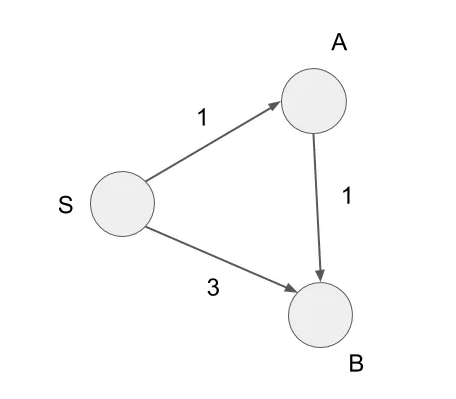
\includegraphics[width=0.6\linewidth]{images/edge_relaxation.png}    

    \caption{Simple weighted, directed graph, used as a demonstration for edge relaxations. https://towardsdatascience.com/algorithm-shortest-paths-1d8fa3f50769}
    \label{fig:edge_r} 
\end{figure}

As an example, consider the graph in \autoref{fig:edge_r}. If we run Dijkstra's algorithm on this graph with starting vertex \emph{S}, we get distances \emph{A=1} and \emph{B=3} after the first pass. After the second pass however (exploring from vertex \emph{A}), we find an alternate path to \emph{B} (\emph{S->A->B}), the length of which is lower than our tentative distance for \emph{B} (1+1 < 3). Therefore, an \textbf{edge relaxation} is completed as the distance is updated to \emph{B=2} and the graph is fully explored.

\subsection{KMP}
\cite{a}
The \textbf{Knuth-Morris-Pratt (KMP)} algorithm is a string searching algorithm that efficiently finds all occurrences of a pattern string \emph{P} in a text string \emph{T}. It was developed by Donald Knuth, James H. Morris, and Vaughan Pratt in 1977. The KMP algorithm is widely used in various applications such as text editors, word processors, and compilers.

The basic idea behind the KMP algorithm is to use the information of previous matches to avoid unnecessary character comparisons in the text string. Specifically, it constructs a prefix function that computes the length of the longest proper prefix of P that is also a suffix of each prefix of P. This information is then used to determine the starting position of the next comparison when a mismatch occurs.

The generated questions will ask students to use build a border table, which is required for string pattern matching in KMP.

The following definitions describe important characteristics for this process of building a border table:
\subsubsection{Border}

A border is a non-empty proper prefix of a string that is also a suffix of that string. More formally, let \emph{s} be a string. A border of \emph{s} is a string\emph{b} that satisfies the following two conditions:
\begin{enumerate}
	\item
	\emph{b} is a proper prefix of \emph{s}, i.e., \emph{b} is not equal to \emph{s}.
	\item
	\emph{b} is also a suffix of \emph{s}, i.e., the last few characters of \emph{s} match the first few characters of \emph{b}.
\end{enumerate}
For example, the string "abab" has two borders: "a" and "ab". Both "a" and "ab" are non-empty proper prefixes of "abab" and are also suffixes of "abab".

\subsubsection{Border table}

 A border table is a data structure that stores the lengths of the borders of all prefixes of a given string. It is an array of integers, where each entry \emph{i} corresponds to the length of the longest border of the prefix of the string that ends at position \emph{i}. The first entry of the border table is always zero, since the empty string has no border.

For example, consider the string "ababaca". The border table for this string would be:

\begin{table}[!h]
\begin{center}
\begin{tabular}{|c||c|c|c|c|c|c|c|}
	\hline
	i & 0 & 1 & 2 & 3 & 4 & 5 & 6 \\
	\hline
	s & a & b & a & b & a & c & a \\
	\hline
	B[i] & 0 & 0 & 1 & 2 & 3 & 0 & 1 \\ 
	\hline
\end{tabular}
\caption{\label{tab:b-table}Border table example}
\end{center}
\end{table}


In \autoref{tab:b-table}, the entry B[2] = 1 corresponds to the length of the longest border of the prefix "ab" of the string "ababaca". This border is "a", which has a length of 1. Similarly, the entry B[4] = 3 corresponds to the length of the longest border of the prefix "ababa" of the string "ababaca". This border is "aba", which has a length of 3.

\subsubsection{Overlapping border}
An overlapping border is an informal term for referring to a border of a string where the end of the prefix border and the beginning of the suffix border overlap.

For example, the string "ababa" has a border "aba", where the last \emph{a} in the prefix border and the first \emph{a} in the suffix border refer to the same character in the string. This border would therefore be considered an overlapping border. Note that the overlapping element can be a single character or a longer substring.

\section{Guidance}
\begin{itemize}    
    \item
      Don't give a laundry list of references.
    \item
      Tie everything you say to your problem.
    \item
      Present an argument.
    \item Think critically; weigh up the contribution of the background and put it in context.    
    \item
      \textbf{Don't write a tutorial}; provide background and cite
      references for further information.
\end{itemize}

%==================================================================================================================================
\chapter{Analysis/Requirements}
\label{chap:req}

This chapter introduces the requirements which ought to be fulfilled in order to satisfy the aims set for the project in \autoref{chap:intro}. These requirements are formulated using the research on prior works as well as the terms and concepts defined in \autoref{chap:back}. As the project essentially has two different products (the program which teachers use to generate and the exercises/solutions themselves given to students), separate requirements must be designed accordingly.
\section{User Personas}

The two distinct users are clearly highlighted by the following user personas.

\subsection{Teacher}

Lisa is a lecturer of computing science at the University of Glasgow. She is teaching a third year undergraduate algorithmics course, which prominently features graph and string search algorithms (such as Dijkstra and KMP). From years of experience having taught this course, Lisa has noticed an increased amount of student collusion during class tests which have been held online since the start of the COVID-19 pandemic. In order to address this, she is seeking a feasible solution which lets her provide each student with a class test comprised of unique examples of exercises. As upholding academic integrity is her main priority, these exercises must be uniform in difficulty but also different enough so that collusion is avoided. From a practicality standpoint, she cannot design this many papers by hand, as the course has over 150 students, therefore exercises must be automatically generated in a format that is easily distributable. To save even more time, Lisa would prefer to have automatically generated step-by-step solutions as well, aiding not only the marking process but also helping students recognise mistakes they have made. In terms of the generation process, she wants a simple user interface which allows her to have some level of input not only to choose which exercises to generate for and how many examples but also to control the difficulty of each exercise as she desires.

\subsection{Student}

John is a third year computing science students at the University of Glasgow, and is attending Lisa's algorithmics course. He is informed that the course is looking to experiment with automatically generated exercises and solutions. While he is open to the idea, he feels strongly about certain features that the system needs to have in order to be feasible. First of all, he believes that that the generated exercise must be visually clear, so that they are not unnecessarily more difficult to solve than hand written ones. In a similar vein, John feels that the exercises should be similar both visually and in content to in-class exercises he has experience with, so that they apply well to the course and do not cause any added confusion. Furthermore, he requires clear instructions to further ensure a good experience. In terms of the generated solutions, John thinks that if each step is explained in detail, he would be very interested in using them for revision purposes.

\section{Program requirements}

In this section, the requirements for a functional and usable automated exercise generation program are outlined. The MoSCoW method is used to categorise each requirements based on importance, as highlighted below.

\subsubsection{Must Have}

These requirements encapsulate the minimum viable product, thus the program becomes unusable if any of these are not delivered.
\begin{itemize}
	\item
	\emph{Produce exercises for the two chosen algorithms (\textbf{Dijkstra} and \textbf{KMP})}: The program must be able fulfil its main goal, which is to generate examples of exercises for each 		selected algorithm, which are output in some format. Without this feature, the application would have no real use-case. 
	\item
	\emph{Ensure uniform difficulty between generated examples}: There must be algorithms in place to address the trade-off between collusion and uniformity in difficulty, as highlighted in \autoref{sec:aim}. One way of achieving this is through the template based approach as seen being successfully used by \cite{Sad12}, to organise each type of exercise by their unique characteristics, which can in turn be controlled to manipulate difficulty. If this issue is not addressed (random generation), the generated exercise would not uphold academic integrity. Each exercise's characteristics should be controllable by the user.
	\item
	\emph{Generate at least 50 separate examples of exercises in one execution}: The program must be able to generate exercises for an entire cohort of students, which may be around 50 to 300 or more students. Therefore, at the bare minimum 50 samples of exercises need to be able to be produced from a given set of input constraints. This number should be able to be controlled by the user.
	\item
	\emph{Generate unique exercises}: Generated exercises must all be unique, in order to avoid collusion between students. Fortunately due to the high number of input variables involved in this study which can be manipulated, identical exercises are highly unlikely because of entropy \cite{}. Thus, this requirement does not need to be enforced explicitly.
	\item
	\emph{Generate exercises in a reasonable time frame}: If the generation process takes hours to complete, the main purpose of not hand-designing each unique exercise is lost. Therefore, process of exercise generation must be relatively time efficient. 
\end{itemize}

\subsubsection{Should Have}
The features in this section increase the usability of the program significantly but are not strictly required for a functional product.
\begin{itemize}
	\item
	\emph{Basic user interface}: The application should at least have a command line based user interface, where teachers can choose various inputs for their desired generations (number of exercises, difficulty, etc.). Without this feature, users would be required to edit the source code or use command line arguments, both of which cannot be expected from people with limited technical experience. 
	\item
	\emph{Automatic answer key}: Even though the minimum viable product handles generating the exercises themselves,  it does not provide the corresponding solutions to these problems, causing the marking process to be drastically prolonged. Having the program generating these solutions would therefore save a lot of time for teachers. Additionally, users should be able to choose whether or not they require these answer keys to speed up execution times in the cases that they do not.
	\item
	\emph{Generate LaTeX files}: The program should output each generating exercise and solution as its own LaTeX, so that these can be easily distributed to students as a compiled PDF file. Having the exercises only within the program itself would make the distribution process very long as they would have to be screenshot individually.
\end{itemize}
\subsubsection{Could Have}
The requirements in this section are in no way essential to the functionality of the program, however they do improve user experience.
\begin{itemize}
	\item
	\emph{Simple visual user interface}: While command line interfaces offer unmatched simplicity, they can often be difficult to use, slow and confusing. To solve this, a simple \emph{JavaFX}   user interface could be implemented, allowing users to give inputs in a more straightforward manner.
	\item
	\emph{Step by step solutions}: Building on the requirement about solution generation in the previous section, the program could also generate step by step instructions on how to solve a given exercise. These would provide students the tools to self-mark their own solutions, while clarifying any confusions that may occur without having to consult a teacher. Similarly to automatic answer key generation, users should be given the option to opt out, speeding up the runtime.
	\item
	\emph{Generate PDF files}: The generated LaTeX files cannot be viewed directly as they must first be compiled to PDF, PNG or other formats. This process of compiling to a PDF file could be done by the program itself through an API, further automating generation and distribution.
\end{itemize}
\subsubsection{Will Not Have}
Since this project has a strict time limit, some requirements which \emph{Could Have} been implemented but are prioritised lower can be found in this section. Note that these features could be seen as a suitable starting point for future work in this field.
\begin{itemize}
	\item
	\emph{Automatic exercise generation for more than two algorithms}: The obvious way to further develop the program would be by implementing new generation algorithms. This process is made streamlined by the fact that the application was made with scalability in mind, so newly designed algorithms can easily be added in the future.
	\item
	\emph{Refined user interface}: As the program evolves with more generation algorithms being added, there comes a point where a simple user interface no longer suffices. At this stage, a system-wide visual overhaul may be considered, perhaps including switching to a web based platform, in order to be more accessible to teachers worldwide. 
	\item
	\emph{Automatic feedback generation}: The third major area of automated exercise generation is automatic \emph{feedback} generation as highlighted by \cite{}. This process involves an entirely different approach to anything tackled in this project, as the inputs change to students' answers, which are automatically reviewed and given feedback. Therefore, this area could be the subject of an entirely new study.
\end{itemize}

%Perhaps something about accessibility
\section{Generated exercise and solution requirements}

In this section, requirements for the generated exercises and solutions can be found, once again categorised by the MoSCoW method. Many characteristics are shared between Dijkstra and KMP which comprise the \emph{Shared Requirements} section, however they both have unique features as well, which are listed separately.

\subsection{Shared requirements}
\subsubsection{Must Have}
\begin{itemize}
	\item
	\emph{Solvable exercises}: The exercises which are generated must have a unique solution, otherwise they would cause a lot of ambiguity if they were to be used in an examination setting. For example, a graph generated for a Dijkstra exercise must be undirected, weighted and connected. Furthermore, there cannot exist any errors such as duplicate edges or weights between two vertices.
\end{itemize}
\subsubsection{Should Have}
\begin{itemize}
	\item
	\emph{Correct Solutions}: For both standard and step-by-step solutions, they should give correct answers to their corresponding exercises. Without this, solutions become redundant.
	\item
	\emph{Clear instructions}: Exercises should have clear instructions for what they are asking of the students, using language based on existing examples of exercises. This is done to ensure that there is no added confusion as a result of automatic generation.
	\item
	\emph{Step description}: In step-by-step solutions, it is often not enough to show the intermediate output of the algorithm, as these can sometimes be confusing. To address this, the solutions should include a short description of what is being done at each step, making it easier for students to follow along. 
	\item
	\emph{Familiar visuals}: The visuals of all exercises and solutions should look similar past exams or in-class examples. This is a necessity for ensuring that no extra burden is being put on students compared to traditional examinations. 
\end{itemize}
\subsubsection{Could Have}
\subsubsection{Will Not Have}
\subsection{Dijkstra Requirements}
\subsubsection{Must Have}
\begin{itemize}
	\item
	\emph{Labelled vertices}: Vertices in the generated graph must labelled, as these will be used as reference in the answer key as well as in students' solutions. 
	\item
	\emph{Edges with weight labels}: As Dijkstra's algorithm requires a weighted graph, the edges must have weight labels in order for the shortest paths to be calculated.
\end{itemize}
\subsubsection{Should Have}
\begin{itemize}
	\item
	\emph{Answers provided in a table}: As the exercise is asking for the shortest path and length from a chosen vertex to all other vertices, these can be well displayed and tracked in a table where each row corresponds to vertex and the three columns are: vertex label, shortest path and length of path. This also works well in step-by-step solutions, as the table can be updated with each round of the algorithm.
\end{itemize}
\subsubsection{Could Have}
\begin{itemize}
	\item
	\emph{Edge and vertex highlights}: In step-by-step solutions, references could be made to the original graph through highlighting certain edges and/or vertices based on what Dijkstra's algorithm is working on in each pass. This would help students visualise how the algorithm works, without having to back to the graph and figuring out for themselves.
	\item
	\emph{Adjacency matrix}: Examples of graphs with a larger number of vertices and edges, edge weights can sometimes be difficult to read. To solve this issue, the graph's adjacency matrix could be provided with each exercise, offering another points of reference for students. This is a great accessibility feature, as it supports people who visualise matrices easier than graphs.
	\item
	\emph{Highlight edge relaxations}: Since students often struggle with finding and handling edge relaxations \cite{} when using Dijkstra's algorithm, they could be highlighted in the solution table in step-by-step answer keys. This can be done by showing which two paths (with distances) are being compared and whether or not this comparison results in an edge relaxation.
\end{itemize}
\subsubsection{Will Not Have}
\begin{itemize}
	\item
	\emph{Custom edge weight placement}: As mentioned earlier, bigger graphs tend to be harder to read due to overlapping edge weights. This may be solved using a custom algorithm which ensures that they are always visible, however this proved to be slightly too time consuming for the purpose of this project.
\end{itemize}
\subsection{KMP Requirements}
\subsubsection{Must Have}
\begin{itemize}
	\item
	\emph{String with borders}: The one feature that is truly essential for building a border table in KMP is the string itself, which must be built up in a way that it corresponds to the teacher's inputs and has borders which can be found. 
\end{itemize}
\subsubsection{Should Have}
\begin{itemize}
	\item
	\emph{Border table in solutions}: In the case of solution generation, the border table can be updated as the algorithm traverses each character in the string, updating the values as borders are found. This helps students visualise how to arrive at the final border table, which is found at the last step.
\end{itemize}
\subsubsection{Could Have}
\begin{itemize}
	\item
	\emph{Border table highlights}: To further aid with the visualisation of results, the string itself and the border table can be highlighted to represent the progression of the algorithm. This is especially useful when trying to find a specific step of the algorithm, which can now be done in a glance.
	\item
	\emph{Border found highlight}: If a border is ever found, it could also be highlighted (with different visuals to the previous requirement), to show which exact substrings the algorithm is referring to when updating the values of border length. This feature is most useful when dealing with overlapping borders \autoref{}, as these can often be harder to find.
 \end{itemize}
\subsubsection{Will Not Have}
\begin{itemize}
	\item
	\emph{String search}: Since KMP is a string search algorithm, it may be odd to see that the exercises generated do not involve searching for a string. This in fact would require a separate generation algorithm, as it deals with an entirely new type of exercise.
\end{itemize}
\section{Changes to Requirements}

As this project subscribes to an agile development process (\cite{}), there were some changes made to requirements, based on supervisor feedback, changing priorities, and time constraints.

Many of these changes can be found in the \textbf{Will Not Have} sections, as most of these requirements started out as \textbf{Could Have}'s but were unable to be completed due to time pressure. For instance, early on during the design phase of the project, generating for more than two algorithms was considered. This idea was dismissed, since it was decided that refining the existing generation algorithms and adding further features to them would be more beneficial for highlighting the benefits of automatic exercise generation, as opposed to repetitively designing a new algorithm. 

Towards the end of the development cycle, a decision had to be made between implementing a simple user interface for the program or developing step-by-step solution generation, as there was only enough time left for one of them. Following discussions with my supervisor, it was decided that the increased functionality of having step-by-step solutions outweighs the usability advantages of having a dedicated user interface. Furthermore, it was noted that the program does not have enough features to warrant a more sophisticated UI, therefore would only be required once more generation algorithms are implemented. Once the decisions was made, the requirements were updated accordingly.

\section{Guidance}
Make it clear how you derived the constrained form of your problem via a clear and logical process. 

%==================================================================================================================================
\chapter{Design}
\label{chap:des}

This chapter discusses the key design decisions made throughout the project, which aim to create a product that satisfies the requirements drawn up in \autoref{chap:req}. As part of these decisions, the final design will be highlighted along with certain alternatives and why they were rejected.

\section{Template Design}

It became apparent quite early on in the project that ensuring uniform difficulty across exercises is one of the greatest challenges of automated exercise generation. This issue can be handled via the \emph{template-based approach} as used successfully in the past. \citet{Hoz21} suggests that for examples with pre-existing exam questions, these should be searched for syntactical characteristics, which must be kept constant to ensure uniform workloads for students (some of these characteristics would be altered to adjust difficulty based on whichever level is required). This is quite helpful for my own project, as there are quite a few past-paper questions to analyse for Algorithmics 1. \citet{Sad12} sports a similar idea, where specific exercises are given templates which highlight their common features while referencing their variables as parameters or "holes". What both of these papers have in common is that it is essential that exercises are deconstructed into fixed and varying parts to ensure uniform difficulty.

In accordance with the aforementioned ideas, the template-based approach was used to design parameters (which will act as user inputs) for both selected exercises as follows.

\subsection{Dijkstra}

When designing a weighted graph, the three main components we must consider are the number of \emph{vertices}, the number of \emph{edges} and the values of edge \emph{weights}. While we could just take these three as our template parameters, this would result in very little variation between samples, as the only randomisation possible would be to change up the order of the vertices and edges. To go a step further, we must consider the unique characteristic of Dijkstra's algorithm, being the number of \emph{edge relaxations}. Since we wish to control the difficulty of each exercise, this number must be kept uniform for all samples. From here follows that the number of \emph{edges} does not need to be a parameter because it can be derived from the number of \emph{edge relaxations}. In a similar vein, the values of edge \emph{weights} are also redundant as they can be derived from the number of \emph{vertices} (the more \emph{vertices} the higher \emph{weight} values are needed to avoid collisions). This is desirable, as we want to have as few user inputs as possible, to eliminate illegal values and general confusion. Therefore, the template parameters (user inputs) for Dijkstra are as follows:

\subsubsection{Number of vertices}

This is the most straightforward way of manipulating exercise difficulty, since the more \emph{vertices} a graph has, the more time it will take to compute its shortest distances using Dijkstra's algorithm. Therefore, this value must be kept constant for all exercises. 

In terms of the accepted range, it is technically possible to generate for any positive integer, however visualising graphs with more than 20 vertices becomes challenging.

\subsubsection{Number of edge relaxations}

In order to control the exercise difficulty for Dijkstra's algorithm specifically, the number of \emph{edge relaxations} must also be kept uniform. This is because graphs with the same number of \emph{vertices} may require significantly different amounts of efforts to solve for Dijkstra depending on their \emph{edge relaxations}. 


\begin{figure}
    \centering
    \begin{subfigure}[b]{0.49\textwidth}
        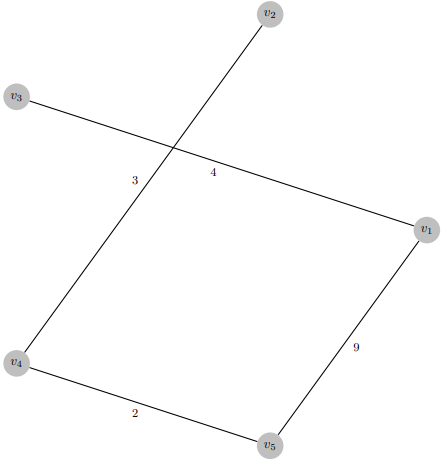
\includegraphics[width=\textwidth]{images/0relax.png}
        \caption{Graph with 5 vertices and 0 edge relaxations from \emph{v1}.}
        \label{fig:0rel}
    \end{subfigure}
    ~ %add desired spacing between images, e. g. ~, \quad, \qquad, \hfill etc. 
      %(or a blank line to force the subfigure onto a new line)
    \begin{subfigure}[b]{0.49\textwidth}
        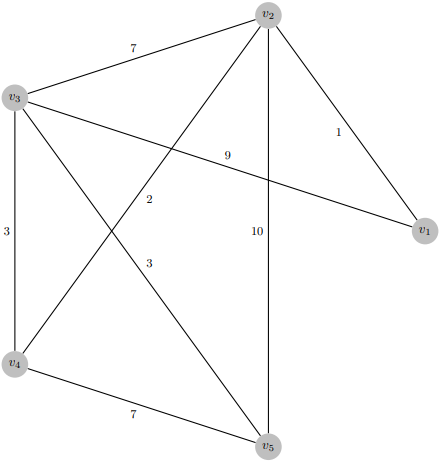
\includegraphics[width=\textwidth]{images/4relax.png}
        \caption{Graph with 5 vertices and 4 edge relaxations from \emph{v1}.}
        \label{fig:4rel}
    \end{subfigure}
    ~ %add desired spacing between images, e. g. ~, \quad, \qquad, \hfill etc. 
    %(or a blank line to force the subfigure onto a new line)    
    \caption{Two random weighted graphs with the same number of vertices (5) but different numbers of edge relaxations (0, 4) from \emph{v1}. Shown side by side to demonstrate how edge relaxations control the number of edges. }\label{fig:relax_compare}
\end{figure}

As shown by \autoref{fig:relax_compare}, the number of \emph{edges} of a graph (4 and 8) is directly correlated to the number of \emph{edge relaxations} (0 and 4 starting from \emph{v1}) when looking at two weighted graphs with the same number of \emph{vertices}. This is because a single \emph{edge relaxation} requires three edges, shown by taking the example of \emph{v1}, \emph{v2}, \emph{v3} from \autoref{fig:4rel}, with \emph{v1} being the starting vertex:
\begin{enumerate}
	\item
	Edge \emph{a} from \emph{v1} to \emph{v2}.
	\item
	Edge \emph{b} from \emph{v1} to \emph{v3}.
	\item
	Edge \emph{c} connecting \emph{v2} to \emph{v3}, where \emph{len(a+c) < len(b)}, causing an edge relaxation.
\end{enumerate}

Thus, adding more \emph{edge relaxations} results in having more \emph{edges}. This means that exercises with more \emph{edge relaxations} are inherently more difficult to solve, as more comparisons are required to be made due to the higher number of \emph{edges}, let alone considering the effort needed to keep updating the shortest distances. 

The minimum number of edge relaxations is 0, while the maximum \emph{r} for a graph with number of vertices \emph{v} and \emph{n=v-2} is:

\begin{equation}
	\label{eq:relax}
	r = \frac{n (n + 1)}{2}
\end{equation}

This follows from the fact that (if inserting in order) after the second vertex (graphs with 0, 1 and 2 vertices cannot have any edge relaxations, hence the \emph{n=v-2}), each additional vertex provides the possibility of one more edge relaxation than its predecessor (third vertex can have one by connecting it to the first, fourth vertex can have two by connecting to the first and second, etc.). This corresponds the series of the sum of natural numbers \cite{a}, with \autoref{eq:relax}.

From these two parameters, other characteristics of Dijkstra's algorithm can be acquired in the following way:

\subsubsection{Number of edges}

As previously described, the number of edges is directly controlled by the number of edge relaxations parameter, therefore it gets adjusted automatically by the generation algorithm, thus it cannot be an input variable. Furthermore, having the number of edges as user input along with the number of edge relaxations would cause many input errors, as graphs with many edge relaxations require more edges by design. 

\subsubsection{Edge weights}

This leaves the challenge of what values to assign to each edge weight. While this could also be a user input (maximum weight, distribution, etc.), we want to keep the generated exercises as simple arithmetically as possible (keep the student's efforts focused on Dijkstra's algorithm) and want to minimise the number of input variables, therefore this can also be handled internally. In essence, there is no hard limit to the values of the weights but they are weakly correlated to the number of vertices, as larger graphs require higher weight values to avoid overlapping when it comes to generating edge relaxations. Furthermore, edges weights have certain limitations to satisfy the number of edge relaxations required, therefore they must be assigned by the algorithm. This process is further explained when exploring the Dijkstra exercise generation algorithm in \autoref{sec:dgen}. 

\subsection{KMP}

To arrive at a string from which a border table can be constructed, there are countless user inputs (template parameters) which may be considered. However, we want to optimise this number to minimise the moving parts accessible by users (avoid input errors) while still providing teachers with ample control over the difficulties of the generated exercises. Keeping this in mind, the following parameters were chosen as user input from reviewing existing KMP exercises.

\subsubsection{String size}

The most straightforward characteristics of a string in KMP is its length. This must be controlled, as the longer the input string, the more effort it will take students to construct its border table. Having this be a fixed input does not cause any issues, as the content of the string can still be randomised to give ample variation between generated samples.

This input must be a natural number, however larger number may be more difficult to visualise.

\subsubsection{Largest border size}

Since it is very complex to control the entire distribution of borders which make up a string, the next best thing is focus on border which causes the most trouble for students, being the largest one. 

\subsubsection{Overlapping or Non-overlapping largest border}

The following characteristics could have been considered as user inputs, however were omitted due to reasons explained below.

\subsubsection{Alphabet}


\section{Generation Algorithm Design}

\subsection{Dijkstra}
\label{sec:dgen}
\subsection{KMP}

\section{User Interface Design}

\section{Exercise and Solution Design}

\subsection{Dijkstra}
\subsection{KMP}

\section{Technologies}

\subsection{Java}
\subsection{LaTeX}

\section{Guidance}
Design should cover the abstract design in such a way that someone else might be able to do what you did, but with a different language or library or tool.

%==================================================================================================================================
\chapter{Implementation}
\label{chap:imp}
What did you do to implement this idea, and what technical achievements did you make?
\section{Guidance}
You can't talk about everything. Cover the high level first, then cover important, relevant or impressive details.



\section{General points}

These points apply to the whole dissertation, not just this chapter.



\subsection{Figures}
\emph{Always} refer to figures included, like Figure \ref{fig:relu}, in the body of the text. Include full, explanatory captions and make sure the figures look good on the page.
You may include multiple figures in one float, as in Figure \ref{fig:synthetic}, using \texttt{subcaption}, which is enabled in the template.



% Figures are important. Use them well.
\begin{figure}
    \centering
    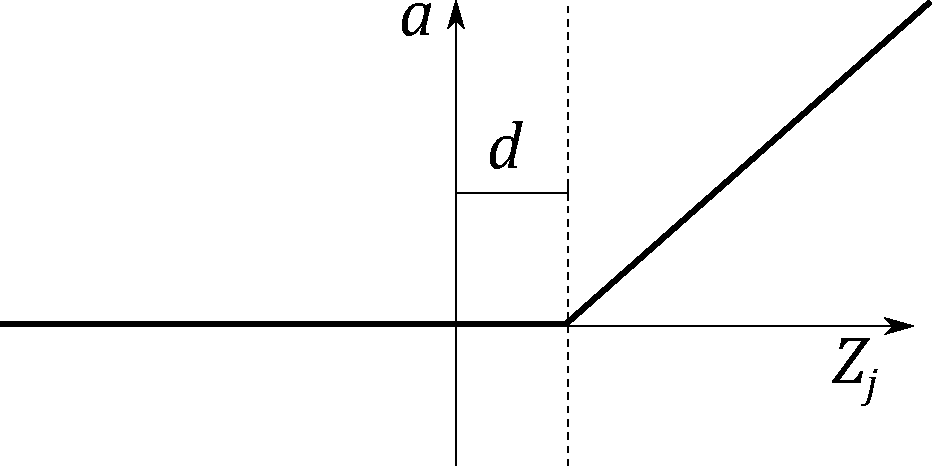
\includegraphics[width=0.5\linewidth]{images/relu.pdf}    

    \caption{In figure captions, explain what the reader is looking at: ``A schematic of the rectifying linear unit, where $a$ is the output amplitude,
    $d$ is a configurable dead-zone, and $Z_j$ is the input signal'', as well as why the reader is looking at this: 
    ``It is notable that there is no activation \emph{at all} below 0, which explains our initial results.'' 
    \textbf{Use vector image formats (.pdf) where possible}. Size figures appropriately, and do not make them over-large or too small to read.
    }

    % use the notation fig:name to cross reference a figure
    \label{fig:relu} 
\end{figure}


\begin{figure}
    \centering
    \begin{subfigure}[b]{0.45\textwidth}
        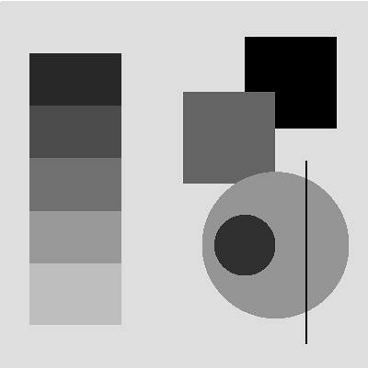
\includegraphics[width=\textwidth]{images/synthetic.png}
        \caption{Synthetic image, black on white.}
        \label{fig:syn1}
    \end{subfigure}
    ~ %add desired spacing between images, e. g. ~, \quad, \qquad, \hfill etc. 
      %(or a blank line to force the subfigure onto a new line)
    \begin{subfigure}[b]{0.45\textwidth}
        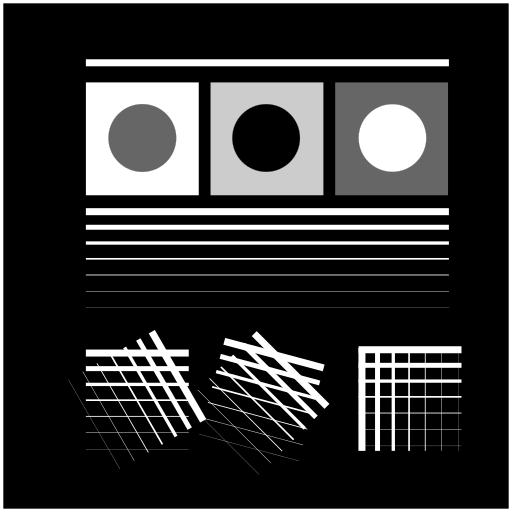
\includegraphics[width=\textwidth]{images/synthetic_2.png}
        \caption{Synthetic image, white on black.}
        \label{fig:syn2}
    \end{subfigure}
    ~ %add desired spacing between images, e. g. ~, \quad, \qquad, \hfill etc. 
    %(or a blank line to force the subfigure onto a new line)    
    \caption{Synthetic test images for edge detection algorithms. \subref{fig:syn1} shows various gray levels that require an adaptive algorithm. \subref{fig:syn2}
    shows more challenging edge detection tests that have crossing lines. Fusing these into full segments typically requires algorithms like the Hough transform.
    This is an example of using subfigures, with \texttt{subref}s in the caption.
    }\label{fig:synthetic}
\end{figure}

\clearpage

\subsection{Equations}

Equations should be typeset correctly and precisely. Make sure you get parenthesis sizing correct, and punctuate equations correctly 
(the comma is important and goes \textit{inside} the equation block). Explain any symbols used clearly if not defined earlier. 

For example, we might define:
\begin{equation}
    \hat{f}(\xi) = \frac{1}{2}\left[ \int_{-\infty}^{\infty} f(x) e^{2\pi i x \xi} \right],
\end{equation}    
where $\hat{f}(\xi)$ is the Fourier transform of the time domain signal $f(x)$.

\subsection{Algorithms}
Algorithms can be set using \texttt{algorithm2e}, as in Algorithm \ref{alg:metropolis}.

% NOTE: line ends are denoted by \; in algorithm2e
\begin{algorithm}
    \DontPrintSemicolon
    \KwData{$f_X(x)$, a probability density function returing the density at $x$.\; $\sigma$ a standard deviation specifying the spread of the proposal distribution.\;
    $x_0$, an initial starting condition.}
    \KwResult{$s=[x_1, x_2, \dots, x_n]$, $n$ samples approximately drawn from a distribution with PDF $f_X(x)$.}
    \Begin{
        $s \longleftarrow []$\;
        $p \longleftarrow f_X(x)$\;
        $i \longleftarrow 0$\;
        \While{$i < n$}
        {
            $x^\prime \longleftarrow \mathcal{N}(x, \sigma^2)$\;
            $p^\prime \longleftarrow f_X(x^\prime)$\;
            $a \longleftarrow \frac{p^\prime}{p}$\;
            $r \longleftarrow U(0,1)$\;
            \If{$r<a$}
            {
                $x \longleftarrow x^\prime$\;
                $p \longleftarrow f_X(x)$\;
                $i \longleftarrow i+1$\;
                append $x$ to $s$\;
            }
        }
    }
    
\caption{The Metropolis-Hastings MCMC algorithm for drawing samples from arbitrary probability distributions, 
specialised for normal proposal distributions $q(x^\prime|x) = \mathcal{N}(x, \sigma^2)$. The symmetry of the normal distribution means the acceptance rule takes the simplified form.}\label{alg:metropolis}
\end{algorithm}

\subsection{Tables}

If you need to include tables, like Table \ref{tab:operators}, use a tool like https://www.tablesgenerator.com/ to generate the table as it is
extremely tedious otherwise. 

\begin{table}[]
    \caption{The standard table of operators in Python, along with their functional equivalents from the \texttt{operator} package. Note that table
    captions go above the table, not below. Do not add additional rules/lines to tables. }\label{tab:operators}
    %\tt 
    \rowcolors{2}{}{gray!3}
    \begin{tabular}{@{}lll@{}}
    %\toprule
    \textbf{Operation}    & \textbf{Syntax}                & \textbf{Function}                            \\ %\midrule % optional rule for header
    Addition              & \texttt{a + b}                          & \texttt{add(a, b)}                                    \\
    Concatenation         & \texttt{seq1 + seq2}                    & \texttt{concat(seq1, seq2)}                           \\
    Containment Test      & \texttt{obj in seq}                     & \texttt{contains(seq, obj)}                           \\
    Division              & \texttt{a / b}                          & \texttt{div(a, b) }  \\
    Division              & \texttt{a / b}                          & \texttt{truediv(a, b) } \\
    Division              & \texttt{a // b}                         & \texttt{floordiv(a, b)}                               \\
    Bitwise And           & \texttt{a \& b}                         & \texttt{and\_(a, b)}                                  \\
    Bitwise Exclusive Or  & \texttt{a \textasciicircum b}           & \texttt{xor(a, b)}                                    \\
    Bitwise Inversion     & \texttt{$\sim$a}                        & \texttt{invert(a)}                                    \\
    Bitwise Or            & \texttt{a | b}                          & \texttt{or\_(a, b)}                                   \\
    Exponentiation        & \texttt{a ** b}                         & \texttt{pow(a, b)}                                    \\
    Identity              & \texttt{a is b}                         & \texttt{is\_(a, b)}                                   \\
    Identity              & \texttt{a is not b}                     & \texttt{is\_not(a, b)}                                \\
    Indexed Assignment    & \texttt{obj{[}k{]} = v}                 & \texttt{setitem(obj, k, v)}                           \\
    Indexed Deletion      & \texttt{del obj{[}k{]}}                 & \texttt{delitem(obj, k)}                              \\
    Indexing              & \texttt{obj{[}k{]}}                     & \texttt{getitem(obj, k)}                              \\
    Left Shift            & \texttt{a \textless{}\textless b}       & \texttt{lshift(a, b)}                                 \\
    Modulo                & \texttt{a \% b}                         & \texttt{mod(a, b)}                                    \\
    Multiplication        & \texttt{a * b}                          & \texttt{mul(a, b)}                                    \\
    Negation (Arithmetic) & \texttt{- a}                            & \texttt{neg(a)}                                       \\
    Negation (Logical)    & \texttt{not a}                          & \texttt{not\_(a)}                                     \\
    Positive              & \texttt{+ a}                            & \texttt{pos(a)}                                       \\
    Right Shift           & \texttt{a \textgreater{}\textgreater b} & \texttt{rshift(a, b)}                                 \\
    Sequence Repetition   & \texttt{seq * i}                        & \texttt{repeat(seq, i)}                               \\
    Slice Assignment      & \texttt{seq{[}i:j{]} = values}          & \texttt{setitem(seq, slice(i, j), values)}            \\
    Slice Deletion        & \texttt{del seq{[}i:j{]}}               & \texttt{delitem(seq, slice(i, j))}                    \\
    Slicing               & \texttt{seq{[}i:j{]}}                   & \texttt{getitem(seq, slice(i, j))}                    \\
    String Formatting     & \texttt{s \% obj}                       & \texttt{mod(s, obj)}                                  \\
    Subtraction           & \texttt{a - b}                          & \texttt{sub(a, b)}                                    \\
    Truth Test            & \texttt{obj}                            & \texttt{truth(obj)}                                   \\
    Ordering              & \texttt{a \textless b}                  & \texttt{lt(a, b)}                                     \\
    Ordering              & \texttt{a \textless{}= b}               & \texttt{le(a, b)}                                     \\
    % \bottomrule
    \end{tabular}
    \end{table}
\subsection{Code}

Avoid putting large blocks of code in the report (more than a page in one block, for example). Use syntax highlighting if possible, as in Listing \ref{lst:callahan}.

\begin{lstlisting}[language=python, float, caption={The algorithm for packing the $3\times 3$ outer-totalistic binary CA successor rule into a 
    $16\times 16\times 16\times 16$ 4 bit lookup table, running an equivalent, notionally 16-state $2\times 2$ CA.}, label=lst:callahan]
    def create_callahan_table(rule="b3s23"):
        """Generate the lookup table for the cells."""        
        s_table = np.zeros((16, 16, 16, 16), dtype=np.uint8)
        birth, survive = parse_rule(rule)

        # generate all 16 bit strings
        for iv in range(65536):
            bv = [(iv >> z) & 1 for z in range(16)]
            a, b, c, d, e, f, g, h, i, j, k, l, m, n, o, p = bv

            # compute next state of the inner 2x2
            nw = apply_rule(f, a, b, c, e, g, i, j, k)
            ne = apply_rule(g, b, c, d, f, h, j, k, l)
            sw = apply_rule(j, e, f, g, i, k, m, n, o)
            se = apply_rule(k, f, g, h, j, l, n, o, p)

            # compute the index of this 4x4
            nw_code = a | (b << 1) | (e << 2) | (f << 3)
            ne_code = c | (d << 1) | (g << 2) | (h << 3)
            sw_code = i | (j << 1) | (m << 2) | (n << 3)
            se_code = k | (l << 1) | (o << 2) | (p << 3)

            # compute the state for the 2x2
            next_code = nw | (ne << 1) | (sw << 2) | (se << 3)

            # get the 4x4 index, and write into the table
            s_table[nw_code, ne_code, sw_code, se_code] = next_code

        return s_table

\end{lstlisting}

%==================================================================================================================================
\chapter{Evaluation} 
\label{chap:ev}
How good is your solution? How well did you solve the general problem, and what evidence do you have to support that?

\section{Guidance}
\begin{itemize}
    \item
        Ask specific questions that address the general problem.
    \item
        Answer them with precise evidence (graphs, numbers, statistical
        analysis, qualitative analysis).
    \item
        Be fair and be scientific.
    \item
        The key thing is to show that you know how to evaluate your work, not
        that your work is the most amazing product ever.
\end{itemize}

\section{Evidence}
Make sure you present your evidence well. Use appropriate visualisations, reporting techniques and statistical analysis, as appropriate.

If you visualise, follow the basic rules, as illustrated in Figure \ref{fig:boxplot}:
\begin{itemize}
\item Label everything correctly (axis, title, units).
\item Caption thoroughly.
\item Reference in text.
\item \textbf{Include appropriate display of uncertainty (e.g. error bars, Box plot)}
\item Minimize clutter.
\end{itemize}

See the file \texttt{guide\_to\_visualising.pdf} for further information and guidance.

\begin{figure}
    \centering
    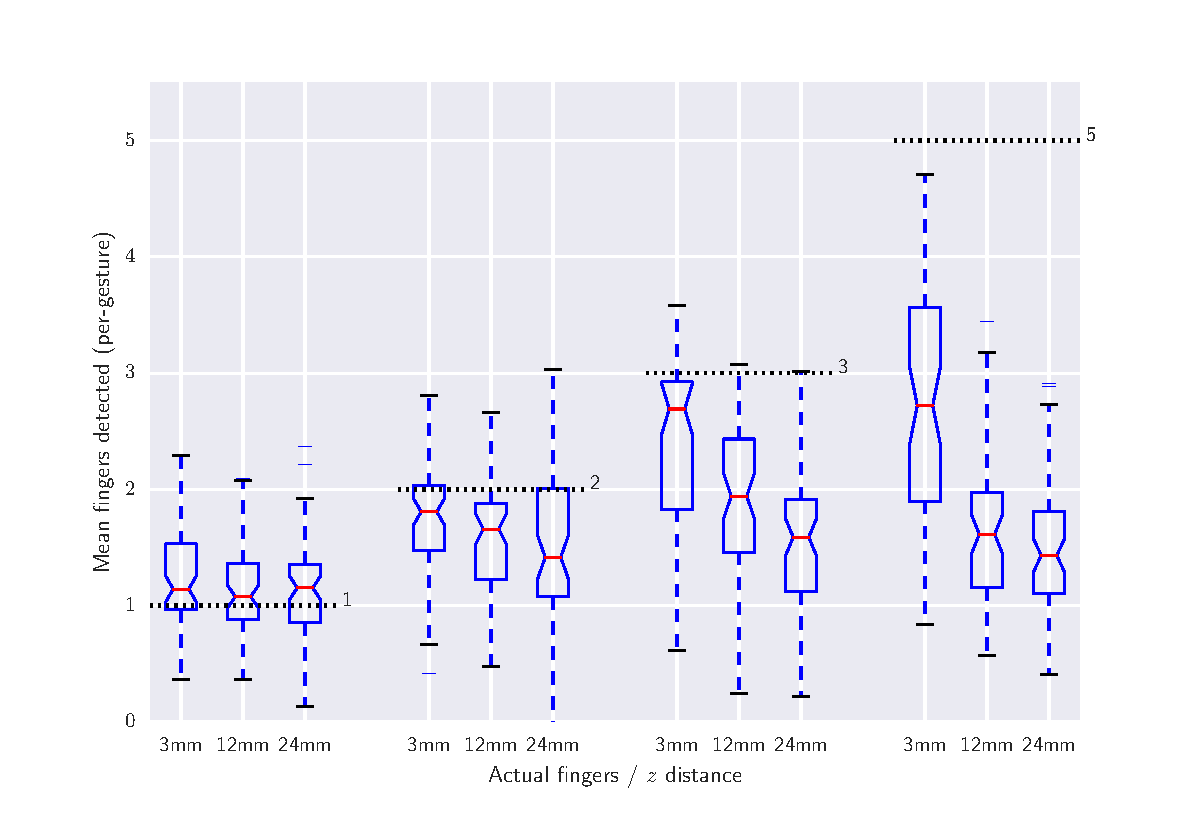
\includegraphics[width=1.0\linewidth]{images/boxplot_finger_distance.pdf}    

    \caption{Average number of fingers detected by the touch sensor at different heights above the surface, averaged over all gestures. Dashed lines indicate
    the true number of fingers present. The Box plots include bootstrapped uncertainty notches for the median. It is clear that the device is biased toward 
    undercounting fingers, particularly at higher $z$ distances.
    }

    % use the notation fig:name to cross reference a figure
    \label{fig:boxplot} 
\end{figure}


%==================================================================================================================================
\chapter{Conclusion}    
\label{chap:conc}
Summarise the whole project for a lazy reader who didn't read the rest (e.g. a prize-awarding committee).
\section{Guidance}
\begin{itemize}
    \item
        Summarise briefly and fairly.
    \item
        You should be addressing the general problem you introduced in the
        Introduction.        
    \item
        Include summary of concrete results (``the new compiler ran 2x
        faster'')
    \item
        Indicate what future work could be done, but remember: \textbf{you
        won't get credit for things you haven't done}.
\end{itemize}

%==================================================================================================================================
%
% 
%==================================================================================================================================
%  APPENDICES  

\begin{appendices}

\chapter{Appendices}

Typical inclusions in the appendices are:

\begin{itemize}
\item
  Copies of ethics approvals (required if obtained)
\item
  Copies of questionnaires etc. used to gather data from subjects.
\item
  Extensive tables or figures that are too bulky to fit in the main body of
  the report, particularly ones that are repetitive and summarised in the body.

\item Outline of the source code (e.g. directory structure), or other architecture documentation like class diagrams.

\item User manuals, and any guides to starting/running the software.

\end{itemize}

\textbf{Don't include your source code in the appendices}. It will be
submitted separately.

\end{appendices}

%==================================================================================================================================
%   BIBLIOGRAPHY   

% The bibliography style is abbrvnat
% The bibliography always appears last, after the appendices.

\bibliographystyle{abbrvnat}

\bibliography{l4proj}

\end{document}
